
%\section{Spectroscopy}

{\color{red} need to smuggle in somewhere that the anisotropic lattices were useful ...}

% set up the ideas of hadron spectro
 
The aim of hadron spectroscopy is to understand the observed experimental spectrum of hadrons in terms of the underlying theory of quarks and gluons, QCD. Traditionally attempts to decipher the regularities present in the spectrum have focussed on models having only limited connection to QCD, but lattice QCD, which offers a first-principles approach to the theory, has now matured to the point where it leads efforts to understand excited hadrons.

In broad terms, one aim of the field is to discover how QCD arranges to have such regularity in the excited spectrum, where the bulk of meson states in accord with excitations of a $q\bar{q}$ system and baryons as $qqq$, and to understand whether or not there are states dominated by configurations of higher numbers of quarks (tetraquarks, pentaquarks), or configurations featuring only glue (glueballs), or excited glue coupled to quarks (hybrids). These latter possibilities, not yet unambiguously observed in experiments, come with potential smoking gun signatures of exotic flavor and/or $J^{PC}$, i.e. quantum numbers not accessible to a simple $q\bar{q}$ system~\cite{Meyer:2015eta}.

Our understanding of the excited hadron spectrum continues to be refined through data obtained in contemporary experimental programs (such as COMPASS, GlueX, CLAS12, BES III, LHCb) which are collecting unprecedented statistics with both established and novel production mechanisms. Observations made by these experiments are introducing new mysteries, such as the ``XYZ'' states in the charmonium region which do not fit into the previously successful modelling of charmonium~\cite{Lebed:2016hpi}.


% now get into lattice

The lightest hadrons such at the neutron, proton, pion, kaon are stable against decay within QCD, and their mass and other properties can be computed with precision within lattice QCD by controlling the systematic uncertainties introduced through the lattice spacing, lattice volume and choice of quark mass. When in addition account is taken of the effects of electromagnetism, excellent agreement is found between theory and experiment~\cite{Duncan:1996xy, Blum:2007cy, Borsanyi:2014jba, Horsley:2015eaa, Blum:2010ym, Aoki:2012st, deDivitiis:2013xla}. {\color{red} these references could certainly be improved, they were culled from a slightly different application}

Unlike these lightest few states, the vast majority of the hadrons which appear in the Particle Data Tables~\cite{Patrignani:2016xqp} are \emph{unstable resonances}, which decay rapidly to lighter hadrons, and whose existence is inferred from enhancements in multi-hadron final states. Decades of accumulated data has led to an experimental spectrum in which each state may be broadly characterized in terms of a mass, a decay width, and branching fractions describing how often the state ends up in each possible decay mode. 

A previous generation of lattice QCD calculations considered the excited hadron spectrum in a simplified manner -- in the case of mesons, a large basis of fermion bilinear operators was used to construct a matrix of correlation functions, which was diagonalized to yield a discrete spectrum of excited state energies. The resulting spectra, determined for isospin=1, isospin=0 and charmonium~\cite{Dudek:2010wm,Dudek:2013yja, Liu:2012ze} show many of the regularities present in the experimental meson spectrum, but also clear signs of \emph{hybrid mesons}, some with exotic $J^{PC}$, not yet observed experimentally.
%{\color{red} could say something about pinning down the hybrid phenomenology from this ... but was in the previous whitepaper}

While these calculations, performed at heavier than physical quark masses, give us a tantalizing glimpse of what lattice QCD can tell us about the hadron spectrum, they are not complete in that the decay physics of the states is not present in any controlled way -- the excited states are appearing as though they were stable states of definite mass rather than as resonances, and the spectrum obtained is at best a guide to the presence of relatively narrow resonances.

In order for a QCD calculation to be faithfully reflecting the physics, it much be capable of resolving excited hadrons as they truly are, as short-lived resonances, typically decaying to more than one final-state. This necessitates the computation of the energy-dependence of coupled-channel scattering amplitudes, in which the resonances will appear as enhancements. In the past five years we have seen significant progress in determining such amplitudes, making use of relations which connect them to the discrete spectrum of eigenstates of quantum field theory in a finite-volume, which can be computed in lattice QCD.

The simplest case is elastic scattering, where in a limited energy region only one hadron-hadron channel in kinematically open. Resonances appearing in elastic scattering include the $\rho$ and the $\sigma$ in $\pi\pi$ scattering, the $K^\star$ in $\pi K$, and the $\Delta$ in $\pi N$, all of which have been considered in lattice QCD
%
~\cite{
%rho
Aoki:2007rd,
Feng:2010es,
Lang:2011mn,
Aoki:2011yj,
Dudek:2012xn,
Pelissier:2012pi,
Wilson:2015dqa,
Bali:2015gji,
Bulava:2016mks,
Guo:2016zos,
% sigma
Briceno:2016mjc,
Guo:2018zss,
% K*
Bali:2015gji, Lang:2012sv, Fu:2012tj, Prelovsek:2013ela,Brett:2018jqw,
% Delta
Andersen:2017una
}.
%
In the elastic case, the scattering amplitude can be described by a single real energy-dependent parameter, the phase-shift, which has a characteristic rise through $90^\circ$ if a narrow resonance is present. Typically for elastic scattering, there is a simple one-to-one mapping of each discrete energy level in a finite-volume to a value of the elastic scattering phase-shift at that energy. It follows that the lattice calculation is required to have a robust determination of the discrete spectrum of eigenstates, ideally in several lattice volumes. Additionally, the use of moving frames and/or asymmetrical volumes, can give access to more energy values which can be used to map out the energy dependence of the phase-shift. To reliably extract the complete spectrum of eigenstates it proves necessary to go beyond the kind of ``single-hadron-like'' operator basis used in the calculation described above, and to also include a set of operators which resemble the relevant hadron-hadron pair undergoing the scattering process.

Developments in the technology of operator and correlation function construction have taken place that mean that these elastic scattering calculations are becoming a commonplace component of a lattice QCD program. Recent examples are presented in Fig~\ref{elastic} for the case of $\pi\pi$ scattering in isospin=1 and isospin=0, where the very different behavior of the $\rho$ resonance and the $\sigma$ can be observed. Lattice QCD~\cite{Briceno:2016mjc} has shown for the first time in a first-principles approach to QCD, that the $\sigma$ meson evolves from being a broad resonance at light quark masses, into a stable bound-state below the $\pi\pi$ threshold, a meson analogue of the deuteron. 

\begin{figure}
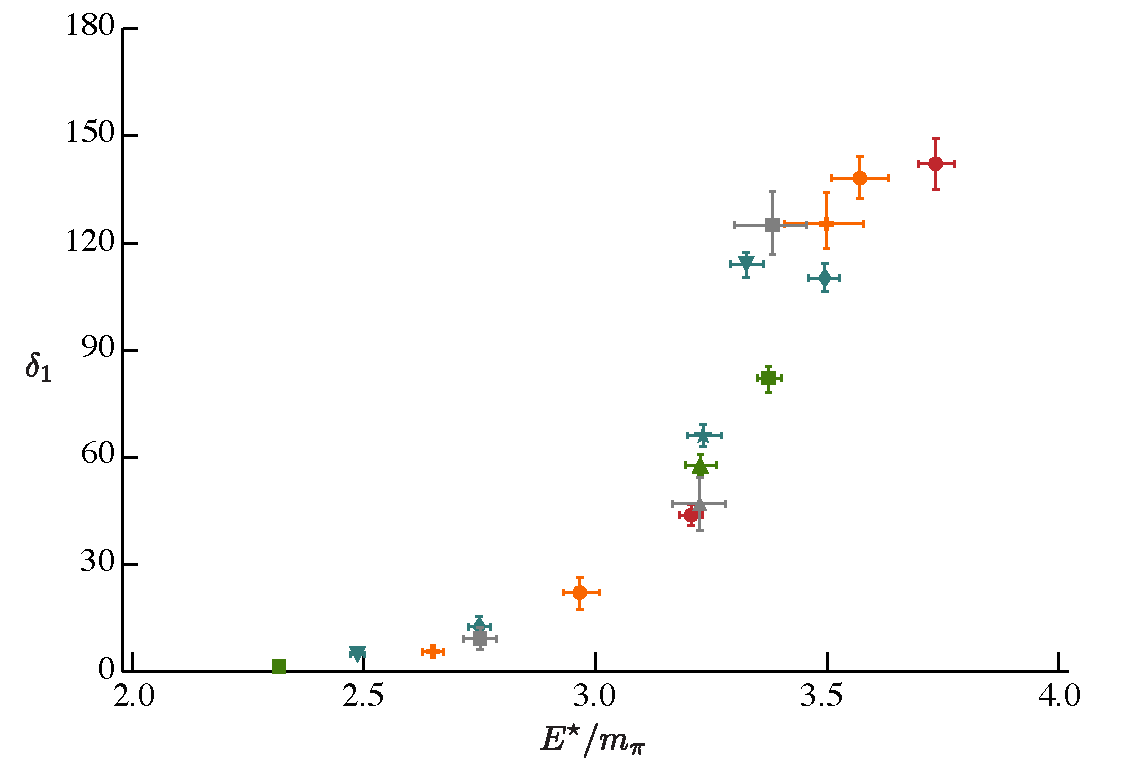
\includegraphics[width=0.44\textwidth]{dudek/bulava}
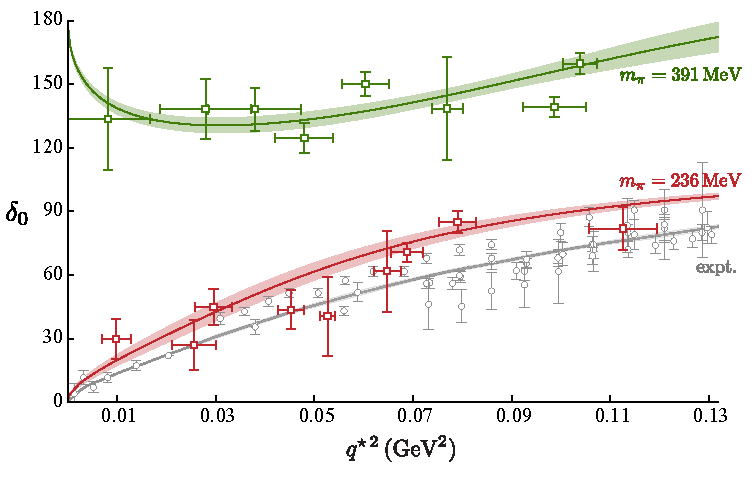
\includegraphics[width=0.48\textwidth]{dudek/sigma}
\caption{$\pi\pi$ elastic scattering phase-shifts from lattice QCD calculations. (a) Isospin=1 $P$-wave computed with $m_\pi \sim 236$ MeV~\cite{Bulava:2016mks} showing the characteristic narrow $\rho$ resonance. (b) Isospin=0 $S$-wave at $m_\pi \sim 391$ MeV and $m_\pi \sim 236$ MeV where the $\sigma$ meson appears as a bound-state, broad resonance respectively~\cite{Briceno:2016mjc}.}
\label{elastic}
\end{figure}


Going beyond the simplest case of elastic scattering, we would intend to compute the coupled-channel $S$-matrix. When more than one hadron-hadron channel is open, the lattice spectrum calculation can be still be done, by extending the operator basis to include hadron-hadron operators of the relevant species, but the analysis to turn this spectrum into information about scattering is less straightforward, since there can no longer be a one-to-one mapping of any given energy level into the multiple unknowns of a coupled-channel scattering matrix at that energy. A successful approach has been to parameterize the energy-dependence of coupled-channel amplitudes, and to use very many discrete energy levels in multiple volumes and/or moving frames to constrain the free parameters. Bias introduced by explicit choice of parameterization can be reduced by considering a range of forms, and exploring to what extent the best-fit amplitudes vary with parameterization choice~\cite{Dudek:2014qha, Wilson:2014cna, Wilson:2015dqa, Moir:2016srx, Dudek:2016cru, Briceno:2017qmb}. 

Having explicit analytic forms for the amplitudes has the advantage that it makes it possible to determine resonance properties in a rigorous way -- by analytically continuing the amplitudes into the complex energy plane, where resonances appear as pole singularities, and where the couplings of resonance states to their decay channels can be obtained from the pole residues.

This methodology was recently used to find low-lying scalar and tensor resonances in the coupled $\pi\pi, K\overline{K}, \eta\eta$ system with isospin=0. In Ref.~\cite{Briceno:2017qmb}, a calculation with pion mass $\sim$ 400 MeV was presented where excited state spectra were extracted from variational analysis of correlation matrices computed in three lattice volumes, in a range of moving frames. The resulting XX energies were used to constrain the amplitudes shown in Figure~\ref{f0f2}. The scalar amplitude has a highly non-trivial behavior in which a bound-state lying below $\pi\pi$ threshold interferes with an $f_0(980)$-like resonance singularity lying close to the $K\overline{K}$ threshold, leading to a \emph{dip} in the $\pi\pi \to \pi \pi$ amplitude that is analogous to a feature seen in the experimental amplitude. The resonance is found to have roughly equal coupling strength to $\pi\pi$ and $K\overline{K}$. The tensor amplitude is quite different, being much closer to our expectations for resonant enhancements, with two clear peaks corresponding to two pole singularities, one coupled dominantly to $\pi\pi$ and the other to $K\overline{K}$ -- numerical estimates are determined for the branching fractions from the pole residues. These two resonances closely resemble the experimentally established $f_2(1270), f_2'(1525)$ states.

This example illustrates the highly non-trivial dynamics that can arise at the level of hadron scattering from the non-perturbative dynamics of QCD, and lattice QCD is for the first time providing us a methodology to explore this dynamics without recourse to poorly motivated approximations or assumptions. {\color{red} ... bit more positive fluff here ...} 

%... also found a0(980) like state ... these scalar mesons long been a problem for simple pictures ... too much detail here ??

A new generation of experiments are studying hadron spectroscopy using novel production mechanisms -- an example being the GlueX experiment at Jefferson Lab, which is producing meson resonances using a photon beam, with a particular focus being the search for exotic $J^{PC}$ hybrid mesons. The anticipated huge data set from this experiment motivates study of the coupling of excited hadrons to photons, and in recent years we have seen the formalism developed to extract the relevant amplitudes from finite-volume lattice QCD calculations, and indeed the first explicit calculation. Refs.~\cite{Briceno:2015dca,Briceno:2016kkp} computed three-point vector current correlation   functions corresponding to the quantum numbers of the process $\gamma^\star \pi \to \pi \pi$ with $J^P=1^-$, in which the $\rho$ resonance is expected to appear. The results of this first calculation with $m_\pi \sim 400$ MeV are presented in Fig~\ref{rhopigamma} where the effect of the $\rho$ resonance in the electromagnetic transition amplitude can be clearly observed, and where the dependence on the virtuality of current can be used to determine the \emph{transition form-factor} of the unstable $\rho$ resonance. A related technology for $e^+ e^-$ annihilation to meson-meson final-states through a photon has also been applied to the elastic $\rho \to \pi\pi$ case~\cite{Feng:2014gba}.

 
\begin{figure}
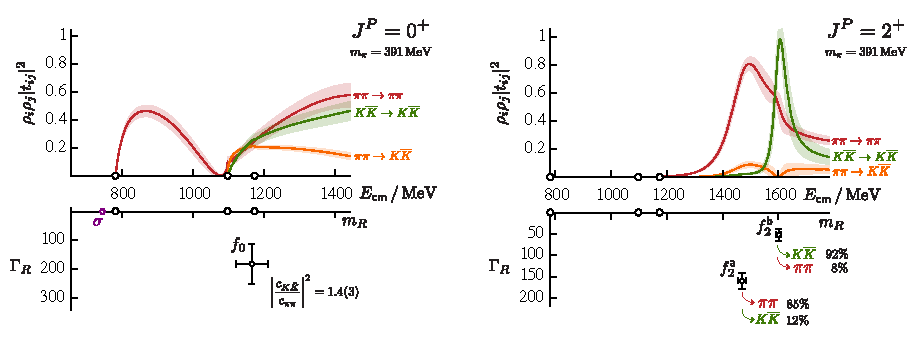
\includegraphics[width=0.8\textwidth]{dudek/f0f2}
\caption{$\pi\pi, K\overline{K}$ coupled-channel scattering amplitudes in two partial-waves determined in a lattice QCD calculation with $m_\pi \sim 391$ MeV~\cite{Briceno:2017qmb}. (a) $J^P=0^+$ sector found to contain a bound-state $\sigma$, but also a resonance pole near the $K\overline{K}$ threshold, having strong coupling to both $K\overline{K}$ and $\pi\pi$ that may be associated with the experimental $f_0(980)$ meson. (b) $J^P=2^+$ sector found to contain two narrow tensor resonances. {\color{red} could prune down the caption}}
\label{f0f2}
\end{figure}


\begin{SCfigure}
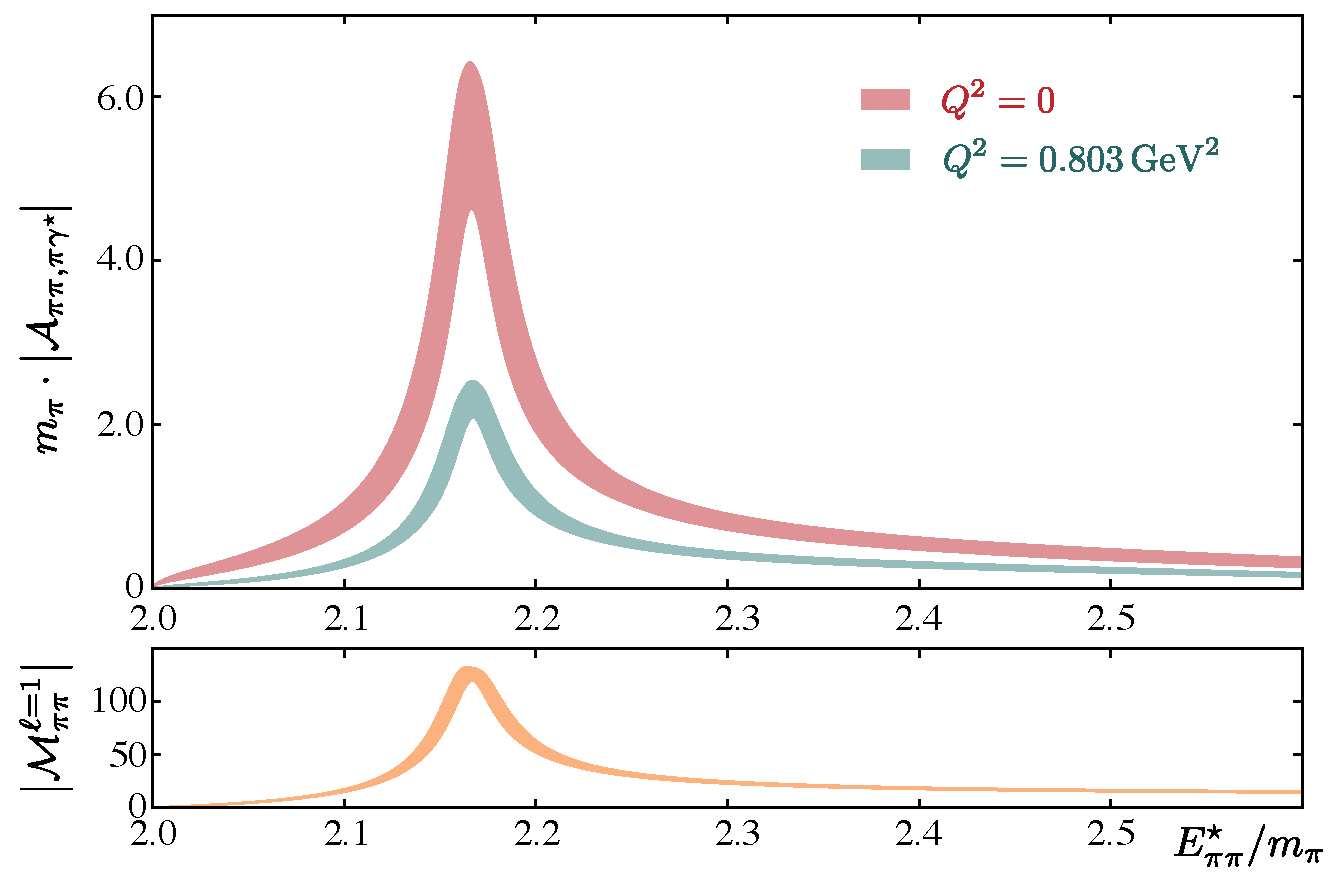
\includegraphics[width=0.45\textwidth]{dudek/rho_pi_gamma}
\caption{Amplitude for the process ${\pi \gamma^\star \to \pi\pi}$ in $P$-wave computed in lattice QCD with $m_\pi \sim 391$ MeV~\cite{Briceno:2016kkp,Briceno:2015dca}. Shown for two values of the photon virtuality, $Q^2$, and also shown the corresponding amplitude for $\pi\pi \to \pi \pi$ indicating that the $\rho$ resonance is contributing to both processes.  }
\label{rhopigamma}
\end{SCfigure}


The progress described above in computation of elastic and coupled-channel scattering and the coupling to scattering systems to external currents has been built upon utilizing large bases of hadron operators, including multi-hadron-like constructions, which typically require the computation of diagrams featuring quark-antiquark annihilation, and these have historically been challenging to include in a statistically precise manner. Techniques such as \emph{distillation}~\cite{Peardon:2009gh} and stochastic variants~\cite{Morningstar:2011ka} {\color{red}( should probably try to cite other suggestions here)} have {\color{red}...}, but with the consequence that the computation cost of the final stage of the lattice calculation, in which the correlation functions are constructed, has become a significant portion of the total computational budget.

{\color{red} ... describe how USQCD resources have made this possible ... }

{\color{red} ... progress called out in NSAC LRP document ... }


\subsection{... future efforts ...}

With the groundwork laid, we expect to see ...

Early targets will see the application of established two-body techniques to channels that have not previously been explored, including the exotic $J^{PC}$ sector in which \emph{hybrid mesons} are predicted to appear. An aim is to predict some properties of these states in advance of the search within the GlueX data set, in particular to offer guidance to their most likely decay channels.


In the short-term, some calculations at heavier than physical quark masses will continue to be warranted. By increasing the light quark mass, pions become heavier, and three-meson thresholds lie higher, providing a larger energy region over which the two-body finite-volume formalism can be applied rigorously. 


Proposed calculations include established meson resonances like $a_1$, $b_1$, which are known to have dominant decays to $\pi \rho$, $\pi \omega$, where at heavier light quark masses, the vector mesons become stable ...

Within the charm sector, the lattice QCD methods described above can be brought to bear on the question of flavor exotics and the other excess `XYZ' states. There have been suggestions that at least some of the observed enhancements arise due to the kinematics of the three-body production process (e.g. $e^+e^- \to J/\psi \, \pi \pi$ or $B \to K \, \psi' \pi$), rather than being due to a true two-body resonance. The lattice calculation has the advantage that it does not need to consider a particular production process, rather it can determine the two-body scattering amplitude directly, and thus investigate the resonance content.
{\color{red} some refs to partial work done ?}

An important current restriction, touched on above, is the absence of a complete formalism to describe three-hadron scattering in a  finite-volume. It is clear that this must be remedied if calculations are to proceed at lighter quark masses, where the bulk of resonances lie above at least one three hadron threshold. A significant formal effort is underway, REFS, ... From the lattice side, the extension of previous calculations is relatively straightforward -- three-hadron-like operators can be constructed using the same techniques used to combine single hadrons into two-hadron operators, and approaches like distillation allow for the relevant correlation functions to be computed. There will naturally be a combinatoric increase in contraction costs, and algorithmic improvements will be explored that seek to reduce these.

While the development of a rigorous three-body (and higher) formalism is vital to have confidence in the calculations of high-lying resonances, it is likely that explicit calculations will show simpler behavior corresponding to quasi-two-body decays. Experimentally resonances appearing in three-body and higher multiplicity final state are observed to dominantly proceed through intermediated two-body states featuring isobar resonances which subsequently decay, e.g. $a_1 \to \rho \pi \to (\pi\pi) \pi$. It may eventually prove possible to make use of this isobar dominance to simplify somewhat the analysis of finite-volume spectra for kinematics with multi-hadron decays.

Most of the developmental work in this field has been done with meson-meson scattering, but in the next five years we expect to see a larger push into the baryon resonance sector. Considering baryon-meson scattering again suffers from a combinatoric increase in contraction cost, but the anticipated algorithmic improvements ... {\color{red} dunno how much to promise here ... the last five year plan was ridiculously optimistic and failed to meet any of its baryon proposals}

Building on the first successful calculations involving currents coupled to resonances, we will see extensions to other resonant states. Transition form-factors evaluated for real photons control the rate of photoproduction at GlueX -- first calculations (even for unphysically heavy quark masses) of established mesons can be compared to the first round of analysis of the GlueX data set, and prediction estimates made for the exotic $J^{PC}$ state production rates. Beyond electromagnetism, we will see calculations of light quark resonances appearing in weak heavy flavor decays {\color{red} ... motivate interest ...}. We can also consider the use of coupling resonances to currents more generally, including currents which are not necessarily experimentally accessible, as a tool to examine the bound structure of resonances. %By computing the current virtuality dependence, and extrapolating to the resonance pole, 

%... charmonium radiative transitions - realistic for above-threshold states ? ... vector decay constants certainly needed ...


... anisotropic physical quark mass ensemble ... first calculations ... elastic resonances ($\rho, \sigma$, $\Delta$) and their couplings to electromagnetism ... 







